\documentclass[10pt,journal,compsoc,onecolumn, draftclsnofoot]{IEEEtran}

\usepackage{graphicx}
\usepackage{amssymb}
\usepackage{amsmath}
\usepackage{amsthm}
\usepackage{caption}

\usepackage{alltt}
\usepackage{float}
\usepackage{color}
\usepackage{url}

\usepackage{balance}
\usepackage[TABBOTCAP, tight]{subfigure}
\usepackage{enumitem}
\usepackage{pstricks, pst-node}

\usepackage{geometry}
\usepackage{pst-gantt}
\usepackage{tabu}

\geometry{textheight=8.5in, textwidth=6in}

%random comment

\newcommand{\cred}[1]{{\color{red}#1}}
\newcommand{\cblue}[1]{{\color{blue}#1}}

\graphicspath{ {images/} }

\usepackage{hyperref}
\usepackage{geometry}
\usepackage{array}
\usepackage{titling}

\def\name{Jake Jeffreys, McKenna Jones, Spike Madden, Sean Marty}
\title{
EmbarkVR: Outdoor Virtual Reality Experience \\
CS Senior Capstone \\
Winter Midterm Progress Report\\
\vspace{1mm}
}
\author{Jake Jeffreys, McKenna Jones, Spike Madden, Sean Marty}
\date{12 Feburary 2016}

%pull in the necessary preamble matter for pygments output

%% The following metadata will show up in the PDF properties
\hypersetup{
  colorlinks = true,
  linkcolor = black,
  urlcolor = black,
  pdfauthor = {\name},
  pdfkeywords = {cs462 ``senior capstone''},
  pdftitle = {CS 462 Progress Report},
  pdfsubject = {CS 462 Progress Report},
  pdfpagemode = UseNone
}

\begin{document}
\begin{titlepage}
\maketitle
\vspace{1mm}
\begin{abstract}
This document describes the progress our group has made over the last term and where will will be going from here. It starts out with a brief overview of the project. It then moves in to discussing problems we encountered and how we able to solve them. Then there is a weekly progress report which breaks down our progress week by week. The document ends with a retrospective and some information related to our plans moving forward.
\end{abstract}
\vspace{1cm}

\noindent\begin{tabular}{ll}
\makebox[2.5in]{\hrulefill} & \makebox[2.5in]{\hrulefill}\\
Intel Sponsor & Date\\[5ex]% adds space between the two sets of signatures
\makebox[2.5in]{\hrulefill} & \makebox[2.5in]{\hrulefill}\\
Columbia Sponsor & Date\\[5ex]% adds space between the two sets of signatures
\makebox[2.5in]{\hrulefill} & \makebox[2.5in]{\hrulefill}\\[2ex]
\makebox[2.5in]{\hrulefill} & \makebox[2.5in]{\hrulefill}\\[2ex]
\makebox[2.5in]{\hrulefill} & \makebox[2.5in]{\hrulefill}\\[2ex]
\makebox[2.5in]{\hrulefill} & \makebox[2.5in]{\hrulefill}\\
Student Team Members & Date\\
\end{tabular}

\end{titlepage}


\tableofcontents
\clearpage


\section{Project Overview}
The current typical retail experience is neither interactive nor immersive.
This project aims to create a functional and immersive virtual reality outdoor experience that promotes Columbia Sportswear gear to outdoor enthusiasts and newcomers alike.
Many outdoor activities initially require a large economic investment to get started.
This makes people less likely to try new outdoor activities.
The goal of the project is to develop an interactive product demonstration to combat this issue by providing customers with an experience of the outdoor activity before they purchase any gear related to it.
This will be accomplished through the use of the HTC Vive and the Unity Game Engine.

The final vision is to have this virtual reality experience placed in a Columbia Sportswear retail store.
Customers will be able to try on apparel in real life, and then perform movements, in the virtual reality experience, while wearing the gear.
This will give customers an idea of how the gear will feel on them when they are performing the same activity in real life.
The primary focus of this project is creating a fishing experience to promote the Performance Fishing Gear line at Columbia Sportswear.

\section{Current Status (McKenna Jones)}
The following section gives insight into where there project currently stands, and the progress we have made since the previous progress report.

\subsection{Previous Work}
During winter break we spent a considerable amount of time becoming familiar with the Unity Game Engine and developing a basic prototype.
This prototype consisted of a basic terrain that would be suitable for our outdoor fishing experience.
This term our work has been a continuation of the progress we made on that prototype.

\subsection{Terrain}
The first area we have worked on is improving the terrain that we created in the prototype.
Originally we simply created an environment that closely resembled a location someone might fish at.
This term we have done a bit more research and roughly based our environment on a few popular fishing destinations around the Pacific NW.
Smith Rock State park in Central Oregon is one of these locations.
Our familiarity with the Unity terrain tools allowed us to do this.
It is fairly easy to use various terrain brushes to sculpt both mountainous and flatter areas.
One can also use the terrain tool to create bushes, trees, grass and other terrain related objects.

\subsection{User Interaction}
The other big area we have been working on is the user interaction aspect of our project, which will be our primary focus from here on out.
The Unity Package, NewtonVR has been the basis of user interaction thus far.
It makes it the process of creating realistic user interaction in a VR environment relatively painless.
You can essentially just add an \textit{InteractableItem} script to any GameObject, and without many adjustments, the user can interact with the item using the HTC Vive wands.
Instead of using the default SteamVR camera within Unity, we are now using the NVRCameraRig, to support this user interaction.
The NewtonVR package also makes it painless to replace the controllers with other objects in the experience.
For example, when the user picks up the fishing rod, the controller model will be replaced with the rod.
The final benefit of NewtonVR is that it makes that objects unable to pass through other objects.
This adds to the realism of the interaction.
Currently we have been working with nailing down the interaction with the fishing rod.
The hardest part of this interaction is making it feel realistic.
Currently we have a rigid fishing rod, and rigid fishing line, which clearly does not look as realistic as we would hope.
Unfortunately, none of us have much experience in this type of work.
We would ideally like there to be a realistic flex to both the rod and the fishing line.
One solution would be to use some type of 3d modeling program like Blender, but this might be out of the scope of this project.
Hopefully we will be able to find an asset on the Unity asset store to solve this issue.

\subsection{Project Focus}
Towards the beginning of this term we came up with the idea to have our VR experience be centered around a campsite.
We figured that this would be the perfect area of showcase some of the Columbia gear.
After talking with out client from Columbia he informed us that they already had a similar experience.
Therefore, we decided it might make more sense to have the experience be focused on user movement.
This way the user can be wearing Columbia gear in real life, while performing actions in VR, like fishing.
This changed our direction slightly, but not dramatically.
We will still keep the campsite, but it will no longer be the main attraction in our environment.

\subsection{Client Interaction}
At this point in the project we have been working with out client to get some essential assets for our project.
Firstly we need Columbia related assets.
This will include different types of apparel from the Performance Fishing Gear line at Columbia.
Ideally these apparel related assets will be ready to be placed on avatars, which our client has suggested is likely.
If this is the case, we hope to have a number of avatars, wearing Columbia gear, that will be walking around the campsite and river to showcase some of the Columbia gear.
We have also been discussing the need for a small budget to purchase some higher quality assets from the Unity Asset Store.
Up until now we have been relying on free assets, which are sufficient, but limit the realism of our experience.
We could focus some of our time on creating our own assets, but this time could be better spent elsewhere, like improving user interaction.

\section{Looking forward (Spike Madden)}
The following sections looks at the tasks that still need to be completed for our virtual reality project.

\subsection{Environment}
We made a lot of progress on the physical environment as most of our developing time has been invested into that. As stated before in the Current Progress section, our VR environment is based off Smith Rock State Park. We're fairly happy with how it's looking right now but have been limited by the use of only free assets.

The layout of the environment is pretty close to what we were envisioning with Smith Rock in mind, but the quality of how realistic the various elements look could be improved. The easiest and best way to handle this would be to use higher quality, most likely paid, assets from Unity's Asset Store. We've compiled a list on our Github wiki that includes the 'Fish School Bundle' by Unlock Software, 'Fishing Gear PACK PBR' by Rokay3D, 'DirectX11 Grass Shader' by Stix Games and 'Camping Site' by Z-Software GmbH. Our Columbia sponsor, Tim Devlin, offered to provide a budget for these assets so we should be getting access to that soon. This is just the first set of assets we determined were necessary and we may look for more improvements over our existing assets in the coming weeks.

Other minor cosmetic changes to textures and shadows can be made to improve realism but it's not our biggest priority right now. We've noticed some frame rate issues but we're unsure whether this is a problem with our development computer's specs or our environment isn't optimized. We'll be looking into this in the coming weeks.

\subsection{Fishing Interaction}
This is the most important component of our project that needs to be completed by the end of this term. There seemed to be a misunderstanding of the project's main goal. As a group, we thought the purpose of this VR experience was to showcase Columbia gear in a fishing experience. However, our sponsors suggested that we focus more on the interactive fishing portion and put less focus on the inclusion and promotion of Columbia products. We sorted this out earlier in the term and we've been putting a bigger emphasis on fishing interaction development.

We've started very preliminary development on the fishing rod and currently have a fishing rod asset with a GameObject attached to it to allow for user interaction. The rod is currently attached to the user's avatar and casts a line with a bobber when the user is near water. This mechanic is still really rough; the rod's positioning is inconsistent, and the fishing line animation is abrupt and unrealistic.

There're several components that we have to improve to create a more realistic fishing experience. From an aesthetics standpoint, having a non-free fishing rod asset would help with the visual presentation. The rod interaction with the controller has to be more fluid in order to maintain immersion. This will be a hard task to accomplish; we need to track the rod accurately and account for the physics of waving the rod around. When near the water, we have to improve the casting animation. The line has to arch in a predictable path based on the user's momentum and movement of the controller. We also need to add fish to the river and the interaction between the rod and fish when the user is fishing. We'll have to think of some mechanism that, when a fish bites, the user can reel back the fish in a realistic manner. There's a lot of work to be done here so most of our time is going to be put into implementing this fishing experience.

\subsection{Columbia Products}
As mentioned in the Fishing Interaction section, we're backing away from the idea of having Columbia gear as the central piece of our VR experience. With that said, our sponsor has mentioned that several Columbia assets are available for use. However, it wasn't really clear from our previous call with Tim what kind of assets would be available. Avatars with Columbia gear with animations would be ideal as it seems unfeasible to attempt to animate the Columbia gear assets on our own.

If we decide to showcase Columbia gear, it would be a minor part of our experience. With the current setup of our campsite area and fishing area, we could place various fishing and camping related products and avatars with Columbia gear for the user to interact with. Anything else seems like it'd be outside of the scope of this project.

\subsection{User Interface}
Creating a basic UI is on our checklist for this project. A launch screen, with 'Enter' and 'Exit' buttons will most likely be the first screen the users encounter. We discussed the idea of an interactive tutorial on the basics of the VR experience but we've left this as a stretch goal for now. The tutorial would introduce the navigation method, campsite and fishing areas, and the fishing mechanics.

We had several requirements for UI relating to Columbia gear, but as our focus has shifted, we're looking into changing them. We had the idea of having product information hover in a panel if a user were to inspect a piece of Columbia apparel or gear. We also had a requirement of a Shopping Cart for Columbia gear but we'll probably leave these features out as the focus of the project changes to be more centered around the fishing experience.

We'll have to create a basic navigation system to let the user move within the experience. To move between the two locations where there's user interaction involved, the campsite area and the fishing area, we'll implement a teleport system that is common in many VR games.

\section{Problems Encountered (Jake Jeffreys)}
Throughout our project we have run into many different issues that have ranged in levels of severity.
Since this is the first time any of us have worked on a Virtual Reality project we knew there would be a lot we would need to overcome.
In this section we have laid out some of the largest issues we have run into so far.

\subsection{Collaboration with Other Virtual Reality Teams}
This year there are multiple senior design teams working on Virtual Reality projects.
During the first couple weeks after getting our project assignments we reached out to individuals on the other teams to start building relationships for future collaboration.
Erik Watterson and his team already had a Vive setup before we received our equipment so he was kind enough to share information related to getting started and ramping up in development.
We got a chance to try out his equipment and he shared some advice related to issues they had run into and overcome.
This ranged from software we would need to download to how to effectively setup the base stations.
This information helped us greatly when we received our gear and were getting started.
Moving forward we were excited about collaborating throughout the project but that’s when some roadblocks appeared.
It turns out that Erik’s group has all signed Nondisclosure Agreements which means they have to be incredibly careful with the information they share.
We attempted to get Nondisclosure agreements for our team so we could begin collaborating but we kept hitting dead ends.
Our two teams collaborated on a few of the reports during the first term but once development began there was very little we could share.
This proved to be quite frustrating because their team had already been working on their project for a few months before the beginning of school at their Intel internship.
This meant that they had more experience than us going into the first term which we could have learned from.
We also could have helped them solve some of there issues.
Instead we had to use online tutorials and just experiment with different techniques until we figured out solutions.

\subsection{Editor View}
None of us had any experience with Virtual Reality or Unity before starting this project but we were all excited to begin development.
The first step was understanding how to interact with Unity and navigate effectively.
There is a large community behind Unity which is super helpful but that doesn’t mean there aren’t some issues with documentation.
One of the first issues we ran into was the rendering distances.
during the development stage where we were placing foliage, the render distances were preventing us from seeing where we had already placed grass.
Fortunately, as we figure out how to better navigatew the editor view, it all become much easier.
This brings up our issue of moving around within the editor.
There was very limited information related to this so we had to figure it out for ourselves through experimentation.
We were able to move around in a relatively mediocre manner but we couldn’t figure out how to move laterally.
After looking at tutorials and on forums we came to the conclusion that it wasn’t a feature they had integrated into Unity yet.
A few weeks later we happened to be working on the project with a different mouse than before and we accidentally pressed down on the scroll wheel.
To our astonishment the whole screened move laterally.
This was incredibly exciting for us and improved our development efficiency exponentially.
We stopped using our mouse pads to do development and now always bring around wireless mice.
It’s unfortunate that this information is so hard to find for new users but we’re glad to have discovered this information relatively early on.

\subsection{Free Asset Availability}
One of the reasons we chose Unity over some of the other gaming engines was the community support behind it.
This makes it a great tool for new developers who have never created virtual reality games before.
It also means there are a wide range of free assets to use.
Towards the beginning of development this was great because we didn’t care as much about quality of assets as we did about building up the terrain and developing user interaction.
Now that our terrain is coming together we have started looking into adding realism to our environment.
This is where some issues have started to arise.
Realism is important to us in this project because we want it to feel as genuine and immersive as possible.
This is when free assets aren’t quite enough.
There are lots of free realism tools and techniques we have taken advantage of but when it comes to close user interaction, the objects need to be highly detailed.
In the world of Unity assets, detail costs money. We began making a list of assets we felt would dramatically improve the realism of our experience such as fishing equipment, fish, and high quality grass renderings.
These are the items that we felt would go the farthest in terms of value.
We then discussed this with our client and they were very open to our ideas.
We hope to get the approval shortly and move on to integrating these assets.

\subsection{Incorporating Columbia Gear}
From the beginning we were under the impression that our project was split between displaying Columbia gear and offering an interactive experience.
We spent a good amount of time brainstorming how to best display Columbia gear and allow user interaction of their clothing lines.
As we started development this term we have been having a hard time getting in contact with our clients to discuss our direction.
During week five we were able to talk with Tim from Columbia to get his input on what we've been working on.
At this point we discovered that Columbia has already worked on some projects that involve showcasing Columbia gear.
We were unaware of this and therefore we were trying to share our time evenly between the two goals.
We needed to change directions slightly and focus more on interactive activities.
Fortunately, we put our heads together and figured out a way to adapt our environment to follow this goal.
We had been working on a campsite to act as a base location and showcase Columbia gear.
Now we are going to keep it as a base and instead allow the user to walk around and interact with general objects.
This adds to immersion and creates a buffer between starting the experience and starting the fishing activity.


\section{Interesting Development Techniques (Sean Marty)}
As with any project, a major portion of the time spent so far has been learning how best to use our tools and what methods give the best results all across the project.
Specifically, our team has been getting better at smoothly moving through the environment in the Unity IDE, integrating our work from different sections into one central project, and adding realism to our landscape.  <-- maybe edit/smooth out this sentence?
This section will break down each of those development technique areas and show how we have implemented them to improve our project.

\subsection{Collaboration}
One of the earliest adaptions we had to make as a team was learning how to get work done when we weren't all on the same development machine.
A good portion of the time we all meet up and work with the laptop provided by Mike Premi and Intel.
However, the wide range of tasks involved means that it is often better to be able to develop on our individual laptops and then merge into one project.
Many teams use Git for their code collaboration, and we have a Github repository for our group.
The problem with using git and Github for managing our project is that the sheer size of the project files makes committing, pushing, and pulling from a remote repository unrealistic.
Also, changes to the project often result in edits to hundreds of asset and configuration files, which can become hard to manage in git.
Our solution is to use the Unity Collaborate Service.
The service is not as widely used or fully featured as Git and Github, but because it is developed for Unity projects specifically, it aligns extremely well with our needs.
The Collaborate tool uses the same basic premise as Github.
The project is stored on the cloud, and users pull and push changes from that location to their local machines.
Commits are tagged with commit messages as in Git, and each time you go to pull new changes down a list of commit messages accompanies the pull.
The beauty of using a Unity service is that the Collaborate tool is already built right into the Unity IDE, and is very simple to download and run.
We have found a lot of success with this tool, and it has allowed for more efficient and varied work.

\subsection{Real Life Environment Basis}
Throughout the entire planning, design, and development of the project we have talked a lot about making the experience realistic.
An environment that is close to a real landscape and better user interaction will make the overall experience feel more immersive.
One of the key ways that we have found to increase realism is through basing our environment on a real place in the world.
The temptation is to just build a landscape that looks good in our minds, but then there is a random collection of plants and trees, rock formations, and other unique parts of the environment.
We chose to match our landscape to pictures of Smith Rock State Park, and so far this has been a great way to make design decisions on many parts of the environment we are building.
There are dozens of ways that we are using this real life location to influence virtual reality choices.
For example, we had built up a basic range of hills around our river valley, but the hills were sort of amorphous and far too symmetrical to be realistic.
After looking through pictures of Smith Rock State Park we were able to redesign the hills to fit the style of rock outcrops we saw, and make the entire landscape's backdrop more meaningful and detailed.
In another part of the project, we changed and updated the vegetation we had placed near the river so that it better matched vegetation near water at Smith Rock.
Both these are examples of bringing a continuity and level of detail to our environment that is extremely important.
For instance, although most users would not specifically comment on a bright green Evergreen tree growing in our dry, dusty environment, the discrepancy would subtly take away from user immersion.
Going forward in development we plan to use real life references for everything that we can, from the fishing activity to how users interact with random objects in the virtual world around them.

\subsection{Unity Tools and Techniques}
Another important part of smooth and efficient development is the ability to move around in and mold our experience in a logical way.
The Unity IDE has some terrific tools for this, and we have learned a lot about how to use them to their full potential.

\subsubsection{Environment Navigation}
The simplest tricks that help with almost all of our development involve navigating through our landscape in the Unity IDE.
There are a bunch of ways to move around the environment, each with a different set of best uses.
The Transform Tools allow panning, rotation, and other basic view modifications.
With the addition of modifier keys, these five buttons provide a long list of ways to interact with the scene.
Mastering how to use these tools has greatly sped up development of the landscape.

\subsubsection{Terrain Tools}
While creating our complex landscape, we made heavy use of Unity's terrain tools.
A terrain object starts as just a flat plane, and then landforms are raised and lowered out of the plane.
We used a couple tricks to make terrain design easier and less repetitive, as well as create better features.
First, we were able to fill every part of our terrain below a certain height with water.
That way, we could carve a riverbed through the middle of our environment, and then fill the river in a way that looked realistic and natural.
Second, the paint height tool allows for some interesting modification to the heightmap of our terrain object.
The paint height tool allows us to sample the height of one area of our terrain and then apply that height to other areas.
This came in handy for aspects such as making a road into the landscape be even and relatively flat, and drawing up flat topped rock formations around the edges of the valley.

\section{Images}
Below are some images that show the current state of our virtual reality experience.

\vspace{1cm}

\begin{figure}[h]
    \centering
    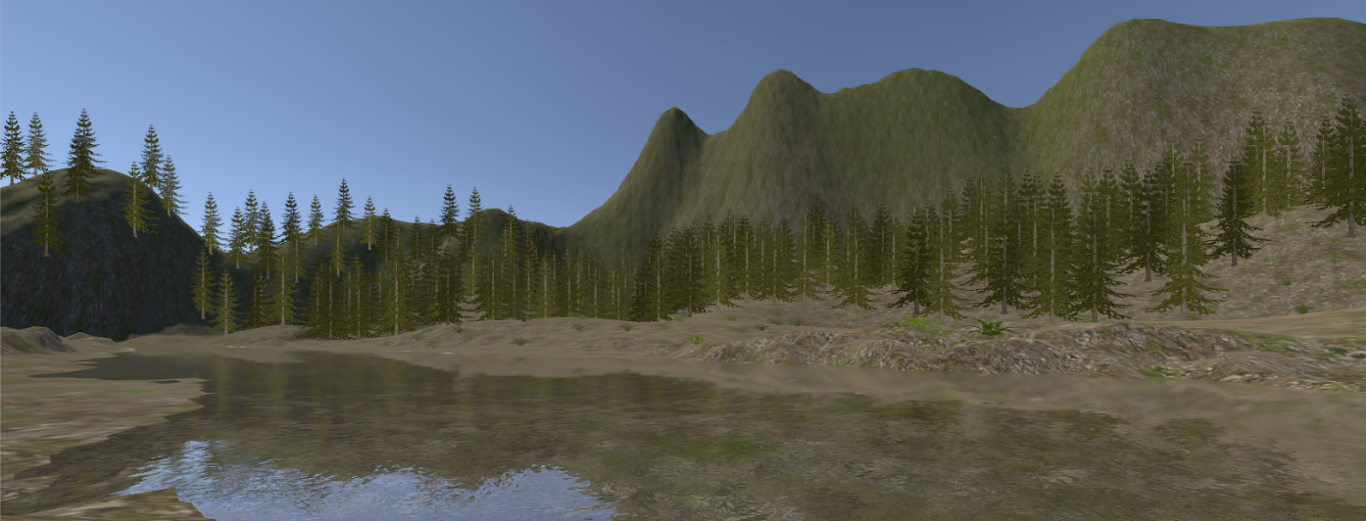
\includegraphics[width=0.75\textwidth]{landscape.png}
    \caption{Image of our landscape}
\end{figure}

\begin{figure}[h]
    \centering
    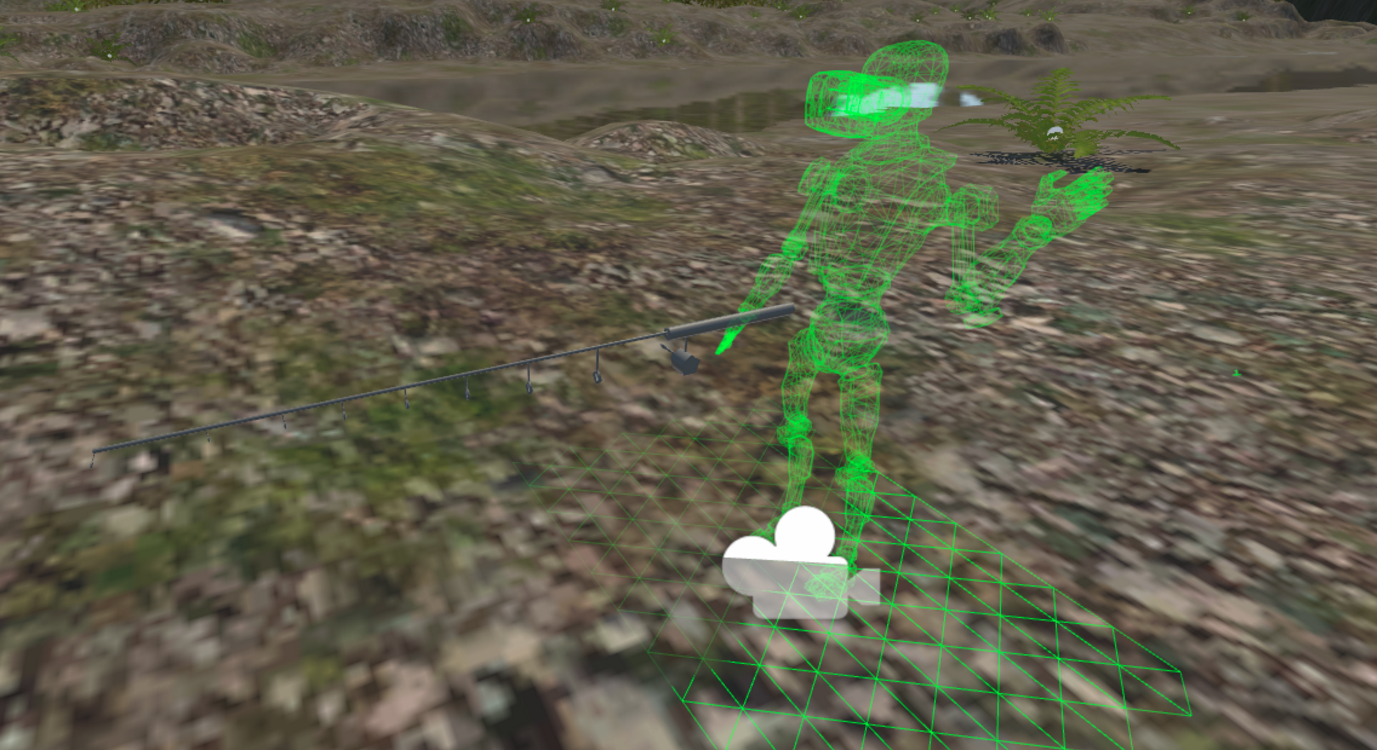
\includegraphics[width=0.75\textwidth]{fishingrod.png}
    \caption{Our virtual reality character with a rough fishing rod and line}
\end{figure}


\end{document}
